\documentclass{ximera}
%% You can put user macros here
%% However, you cannot make new environments

\listfiles

\graphicspath{{./}{firstExample/}{secondExample/}}

\usepackage{tikz}
\usepackage{tkz-euclide}
\usepackage{tikz-3dplot}
\usepackage{tikz-cd}
\usetikzlibrary{shapes.geometric}
\usetikzlibrary{arrows}
\usetkzobj{all}
\pgfplotsset{compat=1.13} % prevents compile error.

%\renewcommand{\vec}[1]{\mathbf{#1}}
\renewcommand{\vec}{\mathbf}
\newcommand{\RR}{\mathbb{R}}
\newcommand{\dfn}{\textit}
\newcommand{\dotp}{\cdot}
\newcommand{\id}{\text{id}}
\newcommand\norm[1]{\left\lVert#1\right\rVert}
 
\newtheorem{general}{Generalization}
\newtheorem{initprob}{Exploration Problem}

\tikzstyle geometryDiagrams=[ultra thick,color=blue!50!black]

%\DefineVerbatimEnvironment{octave}{Verbatim}{numbers=left,frame=lines,label=Octave,labelposition=topline}



\usepackage{mathtools}


\title{How to Use the Modules} \license{CC BY-NC-SA 4.0}



\begin{document}
\begin{abstract}
\end{abstract}
\maketitle



\section*{How to Use the Modules}
Here we will cover some technical aspects of using this text.  In particular, you will learn about the following features:
\begin{itemize}
    \item Machine-graded exercises.
    \item GeoGebra and Desmos interactives.
    \item Saving your work and keeping track of progress.
    \item Data collection.
\end{itemize}

\subsection*{Machine-Graded Exercises}
Machine-graded exercises on the XIMERA platform are designed to help you learn without penalizing you for not getting the right answer the first time.  You can enter answers until you get it right.  
\begin{question}
Try typing $5$ in the answer cell below, then answer the question correctly.
\begin{hint} %  Ha, ha!
    The answer is SMALLER than 5.
\end{hint}
$$2+2=\answer{4}$$
\end{question}
You can enter answers in fraction or in decimal form, as long as your answers are exact.  For example, the following answers are considered equivalent: $\frac{10}{4}=\frac{5}{2}=2.5$.  However, $\frac{1}{3}\neq 0.333$.

\subsection*{GeoGebra and Desmos Interactives}
Embedded GeoGebra and Desmos illustrations allow for added interactivity.
For example, you can use the slider to see where each sample mean fits within the sampling distribution.

\begin{onlineOnly}
\begin{center}
\geogebra{uy3fusxy}{950}{650}
\end{center}
\end{onlineOnly}

\subsection*{Saving your Work and Keeping Track of Progress}
You DO NOT need an account to use XIMERA and save your work.
Your answers will be saved automatically.  If you consistently use the same computer, XIMERA will remember your computer and will keep track of your progress.   WARNING: You will lose your work if you clear out your cookies.

Instructors may require that you submit a proof of completion.  This is easy to do. 
\begin{itemize}
    \item Go to the landing page for the course: \href{https://ximera.osu.edu/qcstats/QC_stats}{Landing Page}
    
\item Click on the ``Certificate" button at the bottom of the page.

\item
Your instructor may ask you to submit a screenshot of your completion summary.
\begin{image}
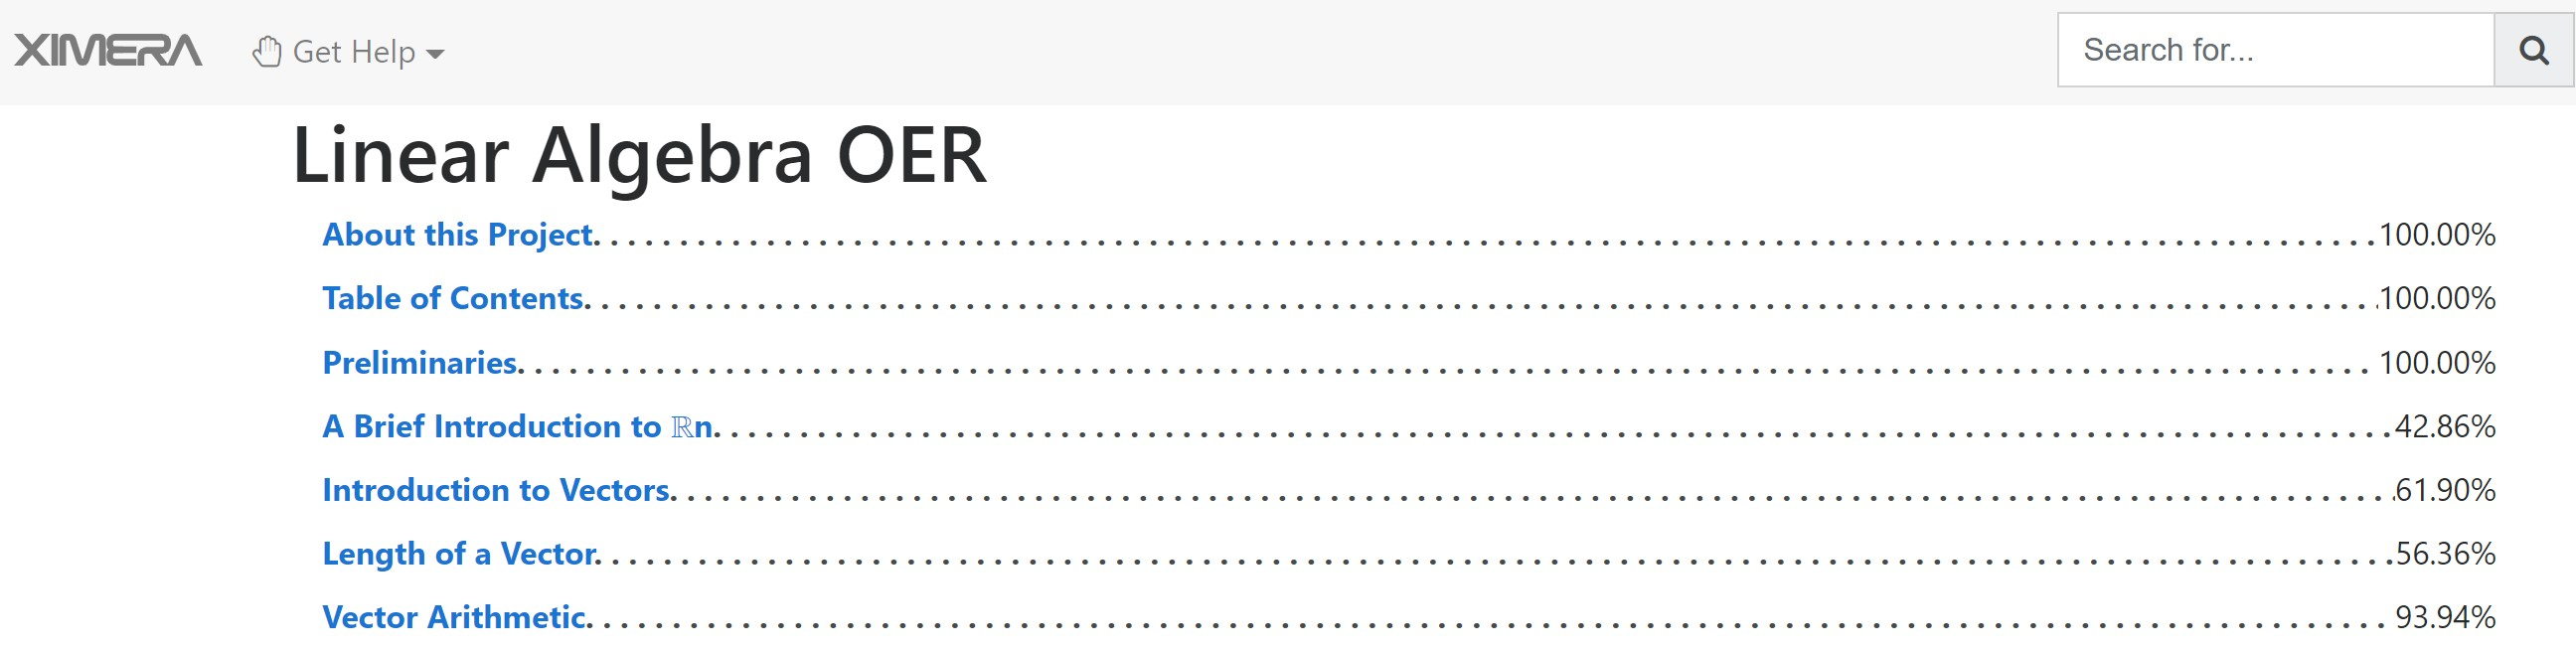
\includegraphics{ximeraScreenshot3.jpg}
\end{image}
\end{itemize}
\subsection*{Data Collection and Usage}
Event stream data from user interactions with the platform -- such as mouse clicks, and submitted answers -- are stored on a secure server at the Ohio State University.  There is no plaintext storage of passwords, and only encrypted protocols for authentication are used.  Anonymized event log is available to the authors of this text through secure access requiring a private key. (GPG is used for this.)   Event log data may be used for research purposes and to improve the product.
\end{document}
